\documentclass{standalone}
\usepackage{tikz}
\usetikzlibrary{arrows.meta}
\begin{document}
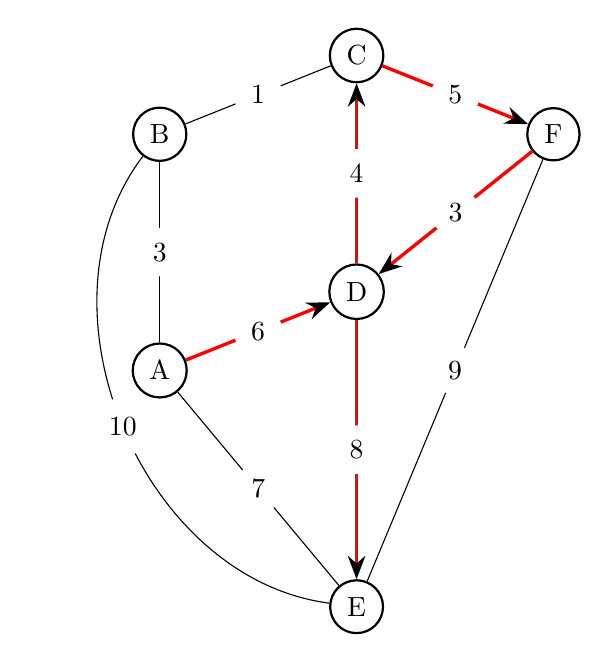
\begin{tikzpicture}
\begin{scope}[every node/.style={circle,thick,draw}]
    \node (A) at (0,0) {A};
    \node (B) at (0,3) {B};
    \node (C) at (2.5,4) {C};
    \node (D) at (2.5,1) {D};
    \node (E) at (2.5,-3) {E};
    \node (F) at (5,3) {F} ;
\end{scope}

\begin{scope}[every node/.style={fill=white,circle}, >={Stealth[black]}]
  \begin{scope}[            
              every edge/.style={draw=red,very thick}]

  \path [->] (A) edge node {$6$} (D);
 \path [->] (D) edge node {$4$} (C);
    \path [->] (C) edge node {$5$} (F);
    \path [->] (F) edge node {$3$} (D);
    \path [->] (D) edge node {$8$} (E);
\end{scope}
    
    \path  (A) edge node {$3$} (B);
    \path  (B) edge node {$1$} (C); 
    \path  (A) edge node {$7$} (E);
    \path  (E) edge node {$9$} (F); 
    \path  (B) edge[bend right=60] node {$10$} (E); 
\end{scope}
\end{tikzpicture}
\end{document}
